% Options for packages loaded elsewhere
\PassOptionsToPackage{unicode}{hyperref}
\PassOptionsToPackage{hyphens}{url}
%
\documentclass[
  oneside]{book}
\usepackage{amsmath,amssymb}
\usepackage{lmodern}
\usepackage{iftex}
\ifPDFTeX
  \usepackage[T1]{fontenc}
  \usepackage[utf8]{inputenc}
  \usepackage{textcomp} % provide euro and other symbols
\else % if luatex or xetex
  \usepackage{unicode-math}
  \defaultfontfeatures{Scale=MatchLowercase}
  \defaultfontfeatures[\rmfamily]{Ligatures=TeX,Scale=1}
\fi
% Use upquote if available, for straight quotes in verbatim environments
\IfFileExists{upquote.sty}{\usepackage{upquote}}{}
\IfFileExists{microtype.sty}{% use microtype if available
  \usepackage[]{microtype}
  \UseMicrotypeSet[protrusion]{basicmath} % disable protrusion for tt fonts
}{}
\makeatletter
\@ifundefined{KOMAClassName}{% if non-KOMA class
  \IfFileExists{parskip.sty}{%
    \usepackage{parskip}
  }{% else
    \setlength{\parindent}{0pt}
    \setlength{\parskip}{6pt plus 2pt minus 1pt}}
}{% if KOMA class
  \KOMAoptions{parskip=half}}
\makeatother
\usepackage{xcolor}
\IfFileExists{xurl.sty}{\usepackage{xurl}}{} % add URL line breaks if available
\IfFileExists{bookmark.sty}{\usepackage{bookmark}}{\usepackage{hyperref}}
\hypersetup{
  pdftitle={Template},
  pdfauthor={psyTeachR Team},
  hidelinks,
  pdfcreator={LaTeX via pandoc}}
\urlstyle{same} % disable monospaced font for URLs
\usepackage[margin=1in]{geometry}
\usepackage{color}
\usepackage{fancyvrb}
\newcommand{\VerbBar}{|}
\newcommand{\VERB}{\Verb[commandchars=\\\{\}]}
\DefineVerbatimEnvironment{Highlighting}{Verbatim}{commandchars=\\\{\}}
% Add ',fontsize=\small' for more characters per line
\usepackage{framed}
\definecolor{shadecolor}{RGB}{248,248,248}
\newenvironment{Shaded}{\begin{snugshade}}{\end{snugshade}}
\newcommand{\AlertTok}[1]{\textcolor[rgb]{0.94,0.16,0.16}{#1}}
\newcommand{\AnnotationTok}[1]{\textcolor[rgb]{0.56,0.35,0.01}{\textbf{\textit{#1}}}}
\newcommand{\AttributeTok}[1]{\textcolor[rgb]{0.77,0.63,0.00}{#1}}
\newcommand{\BaseNTok}[1]{\textcolor[rgb]{0.00,0.00,0.81}{#1}}
\newcommand{\BuiltInTok}[1]{#1}
\newcommand{\CharTok}[1]{\textcolor[rgb]{0.31,0.60,0.02}{#1}}
\newcommand{\CommentTok}[1]{\textcolor[rgb]{0.56,0.35,0.01}{\textit{#1}}}
\newcommand{\CommentVarTok}[1]{\textcolor[rgb]{0.56,0.35,0.01}{\textbf{\textit{#1}}}}
\newcommand{\ConstantTok}[1]{\textcolor[rgb]{0.00,0.00,0.00}{#1}}
\newcommand{\ControlFlowTok}[1]{\textcolor[rgb]{0.13,0.29,0.53}{\textbf{#1}}}
\newcommand{\DataTypeTok}[1]{\textcolor[rgb]{0.13,0.29,0.53}{#1}}
\newcommand{\DecValTok}[1]{\textcolor[rgb]{0.00,0.00,0.81}{#1}}
\newcommand{\DocumentationTok}[1]{\textcolor[rgb]{0.56,0.35,0.01}{\textbf{\textit{#1}}}}
\newcommand{\ErrorTok}[1]{\textcolor[rgb]{0.64,0.00,0.00}{\textbf{#1}}}
\newcommand{\ExtensionTok}[1]{#1}
\newcommand{\FloatTok}[1]{\textcolor[rgb]{0.00,0.00,0.81}{#1}}
\newcommand{\FunctionTok}[1]{\textcolor[rgb]{0.00,0.00,0.00}{#1}}
\newcommand{\ImportTok}[1]{#1}
\newcommand{\InformationTok}[1]{\textcolor[rgb]{0.56,0.35,0.01}{\textbf{\textit{#1}}}}
\newcommand{\KeywordTok}[1]{\textcolor[rgb]{0.13,0.29,0.53}{\textbf{#1}}}
\newcommand{\NormalTok}[1]{#1}
\newcommand{\OperatorTok}[1]{\textcolor[rgb]{0.81,0.36,0.00}{\textbf{#1}}}
\newcommand{\OtherTok}[1]{\textcolor[rgb]{0.56,0.35,0.01}{#1}}
\newcommand{\PreprocessorTok}[1]{\textcolor[rgb]{0.56,0.35,0.01}{\textit{#1}}}
\newcommand{\RegionMarkerTok}[1]{#1}
\newcommand{\SpecialCharTok}[1]{\textcolor[rgb]{0.00,0.00,0.00}{#1}}
\newcommand{\SpecialStringTok}[1]{\textcolor[rgb]{0.31,0.60,0.02}{#1}}
\newcommand{\StringTok}[1]{\textcolor[rgb]{0.31,0.60,0.02}{#1}}
\newcommand{\VariableTok}[1]{\textcolor[rgb]{0.00,0.00,0.00}{#1}}
\newcommand{\VerbatimStringTok}[1]{\textcolor[rgb]{0.31,0.60,0.02}{#1}}
\newcommand{\WarningTok}[1]{\textcolor[rgb]{0.56,0.35,0.01}{\textbf{\textit{#1}}}}
\usepackage{longtable,booktabs,array}
\usepackage{calc} % for calculating minipage widths
% Correct order of tables after \paragraph or \subparagraph
\usepackage{etoolbox}
\makeatletter
\patchcmd\longtable{\par}{\if@noskipsec\mbox{}\fi\par}{}{}
\makeatother
% Allow footnotes in longtable head/foot
\IfFileExists{footnotehyper.sty}{\usepackage{footnotehyper}}{\usepackage{footnote}}
\makesavenoteenv{longtable}
\usepackage{graphicx}
\makeatletter
\def\maxwidth{\ifdim\Gin@nat@width>\linewidth\linewidth\else\Gin@nat@width\fi}
\def\maxheight{\ifdim\Gin@nat@height>\textheight\textheight\else\Gin@nat@height\fi}
\makeatother
% Scale images if necessary, so that they will not overflow the page
% margins by default, and it is still possible to overwrite the defaults
% using explicit options in \includegraphics[width, height, ...]{}
\setkeys{Gin}{width=\maxwidth,height=\maxheight,keepaspectratio}
% Set default figure placement to htbp
\makeatletter
\def\fps@figure{htbp}
\makeatother
\setlength{\emergencystretch}{3em} % prevent overfull lines
\providecommand{\tightlist}{%
  \setlength{\itemsep}{0pt}\setlength{\parskip}{0pt}}
\setcounter{secnumdepth}{5}
\usepackage{booktabs}

\usepackage{tcolorbox}
\usepackage[T1]{fontenc}

\definecolor{dangcol}{RGB}{152,62,130}
\definecolor{warncol}{RGB}{245,220,112}
\definecolor{infocol}{RGB}{70,122,172}
\definecolor{trycol}{RGB}{97,88,156}

\newtcolorbox{dangerous}{
  colback=dangcol!10,
  colframe=dangcol,
  coltext=black,
  boxsep=5pt,
  arc=4pt
}

\newtcolorbox{warning}{
  colback=warncol!10,
  colframe=warncol,
  coltext=black,
  boxsep=5pt,
  arc=4pt
}

\newtcolorbox{info}{
  colback=infocol!10,
  colframe=infocol,
  coltext=black,
  boxsep=5pt,
  arc=4pt
}

\newtcolorbox{try}{
  colback=trycol!10,
  colframe=trycol,
  coltext=black,
  boxsep=5pt,
  arc=4pt
}
\ifLuaTeX
  \usepackage{selnolig}  % disable illegal ligatures
\fi
\usepackage[]{natbib}
\bibliographystyle{plainnat}

\title{Template}
\author{psyTeachR Team}
\date{2021-10-14}

\begin{document}
\maketitle

{
\setcounter{tocdepth}{1}
\tableofcontents
}
\hypertarget{overview}{%
\chapter*{Overview}\label{overview}}
\addcontentsline{toc}{chapter}{Overview}

After copying this template to your project, you will need to change the information in the \texttt{CITATION} and \texttt{DESCRIPTION} files, as well as update the YAML header of \texttt{book/index.Rmd} and \texttt{book/\_output.yml}. Update site-specific logos in \texttt{book/images/logos/}.

If you are not part of the psyTeachR group, please edit the Google Analytics ID in \texttt{include/google-analytics.html} or comment out the relevant line in \texttt{book/\_output.yml}.

Render the book using the code in \texttt{\_render.R}.

\hypertarget{changes}{%
\section{Changes}\label{changes}}

\hypertarget{version-2.1-2021-10-14}{%
\subsection{Version 2.1 2021-10-14}\label{version-2.1-2021-10-14}}

\begin{itemize}
\tightlist
\item
  Updated webexercises styles to include a green check and red X for correct and incorrect responses.

  \begin{itemize}
  \tightlist
  \item
    \texttt{book/include/webex.css} (replace)
  \item
    \texttt{book/include/webex.js} (replace)
  \end{itemize}
\item
  Changed the name of \texttt{book/include/header.html} to \texttt{book/include/google-analytics.html} to better reflect its purpose.

  \begin{itemize}
  \tightlist
  \item
    \texttt{book/include/header.html} (delete)
  \item
    \texttt{book/include/google-analytics.html} (add)
  \item
    \texttt{book/\_output.yml} (change line 10)
  \end{itemize}
\item
  Updated rendering functions to not render pdf epub or mobi by default

  \begin{itemize}
  \tightlist
  \item
    \texttt{\_render.R} (replace)
  \item
    \texttt{Makefile} (add)
  \end{itemize}
\end{itemize}

\hypertarget{inclusion}{%
\chapter{Inclusion}\label{inclusion}}

We want our resources to be accessible to everyone. This means thinking about accessibility with regards to disability, language, identity, and other characteristics. This is a work in progress; feel free to suggest additions.

\hypertarget{tips-for-text-readers}{%
\section{Tips for text-readers}\label{tips-for-text-readers}}

Some students need to use text readers for accessibility; others just prefer this method. Here are some tips for improving their experience from the \href{https://www.bdadyslexia.org.uk/advice/employers/creating-a-dyslexia-friendly-workplace/dyslexia-friendly-style-guide}{Dyslexia Style Guide}.

\begin{itemize}
\tightlist
\item
  Use straight quotation marks
\item
  Avoid roman numerals
\item
  Avoid text in figures
\end{itemize}

Bookdown books allow readers to change the font style, size, and background colour. This provides essential accessibility for some people, such as those with dyslexia or visual impairments. Therefore, avoid putting too much text in figures and provide descriptions of images in the figure caption.

\hypertarget{resources-for-blind-coders}{%
\section{Resources for blind coders}\label{resources-for-blind-coders}}

\begin{itemize}
\tightlist
\item
  \href{https://github.com/ajrgodfrey/BrailleR}{BrailleR}: a collection of tools to make use of R a happier experience for blind people
\item
  \href{https://journal.r-project.org/archive/2013/RJ-2013-007/RJ-2013-007.pdf}{Statistical Software from a Blind Person's Perspective}
\end{itemize}

\hypertarget{dyslexia-friendly-resources}{%
\section{Dyslexia-friendly resources}\label{dyslexia-friendly-resources}}

\begin{itemize}
\tightlist
\item
  \href{https://www.bdadyslexia.org.uk/educator}{British Dyslexia Association}
\item
  \href{https://www.bdadyslexia.org.uk/advice/employers/creating-a-dyslexia-friendly-workplace/dyslexia-friendly-style-guide}{Dyslexia Style Guide}
\item
  \href{https://datacarpentry.org/blog/2017/09/coding-and-dyslexia}{Dyslexia and Coding}: Data Carpentry blog post
\item
  \href{https://cran.r-project.org/web/packages/fcuk/vignettes/fcuk.html}{fcuk}: A package designed to help people with clumsy fingers
\end{itemize}

Some recommendations are highlighted below.

\begin{itemize}
\tightlist
\item
  Avoid underlining, block capitals, and italics -- Use bold instead
\item
  Use \href{conventions.html\#alert-boxes}{boxes and borders} for effective emphasis
\item
  Use left-justified with ragged right edge (don't full-justify)
\item
  Use bullet points and numbering rather than continuous prose
\item
  Use the active voice with concise, direct sentences
\item
  Avoid abbreviations and provide a \href{glossary.html}{glossary} of jargon
\end{itemize}

\hypertarget{colour}{%
\section{Colour}\label{colour}}

You can check your images for how they look to people with different types of colourblindness with the \href{https://www.color-blindness.com/coblis-color-blindness-simulator/}{Coblis Color Blindness Simulator}.

Desi Quintans made \href{https://github.com/DesiQuintans/Pebble-safe}{dark and light colour-blind safe RStudio themes}.

The ``pink'' and ``green'' colours from the \href{}{psyteachr\_colours()} function are distinguishable by people with protanopia (red-blind), deuteronopia (green-blind), and tritanopia (blue-blind) colourblindness. You can also use viridis colours with \texttt{ggplot2::scale\_colour\_viridis\_d()} and \texttt{ggplot2::scale\_fill\_viridis\_d()} (for discrete colours) or \texttt{ggplot2::scale\_colour\_viridis\_c()} and \texttt{ggplot2::scale\_fill\_viridis\_c()} (for continuous colours).

In plots, add secondary indicators in addition to colour, such as text labels or shapes.

\begin{figure}

{\centering 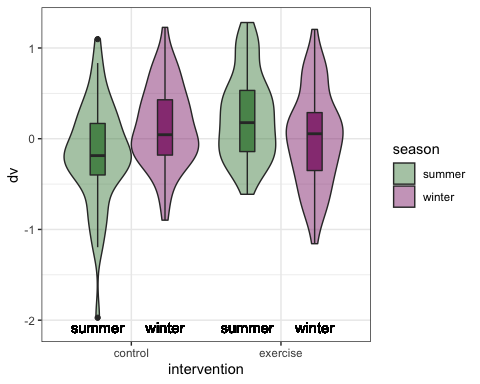
\includegraphics[width=1\linewidth]{01-intro_files/figure-latex/plot-text-labels-1} 

}

\caption{Text labels supplement colour information.}\label{fig:plot-text-labels}
\end{figure}

\begin{figure}

{\centering 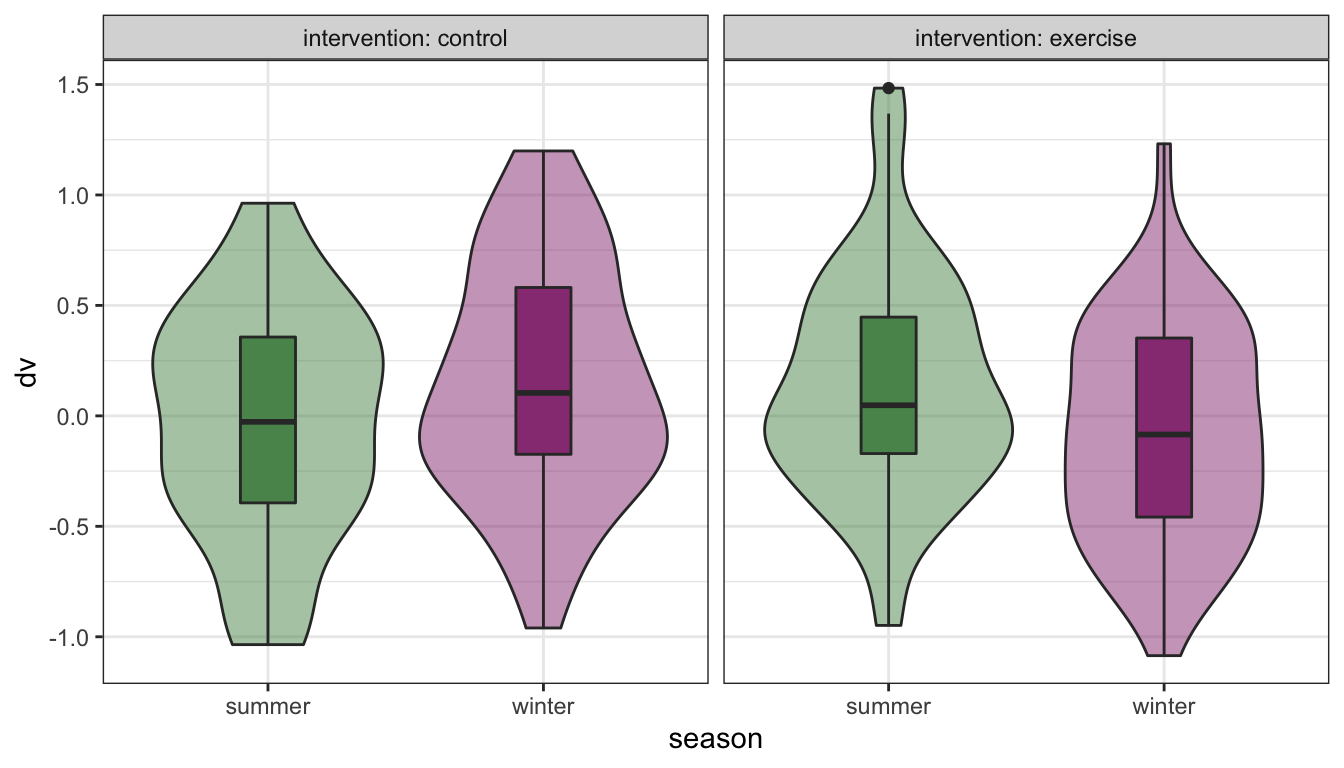
\includegraphics[width=1\linewidth]{01-intro_files/figure-latex/plot-text-labels-facet-1} 

}

\caption{Facet labels and redundant colour information.}\label{fig:plot-text-labels-facet}
\end{figure}

\begin{figure}

{\centering 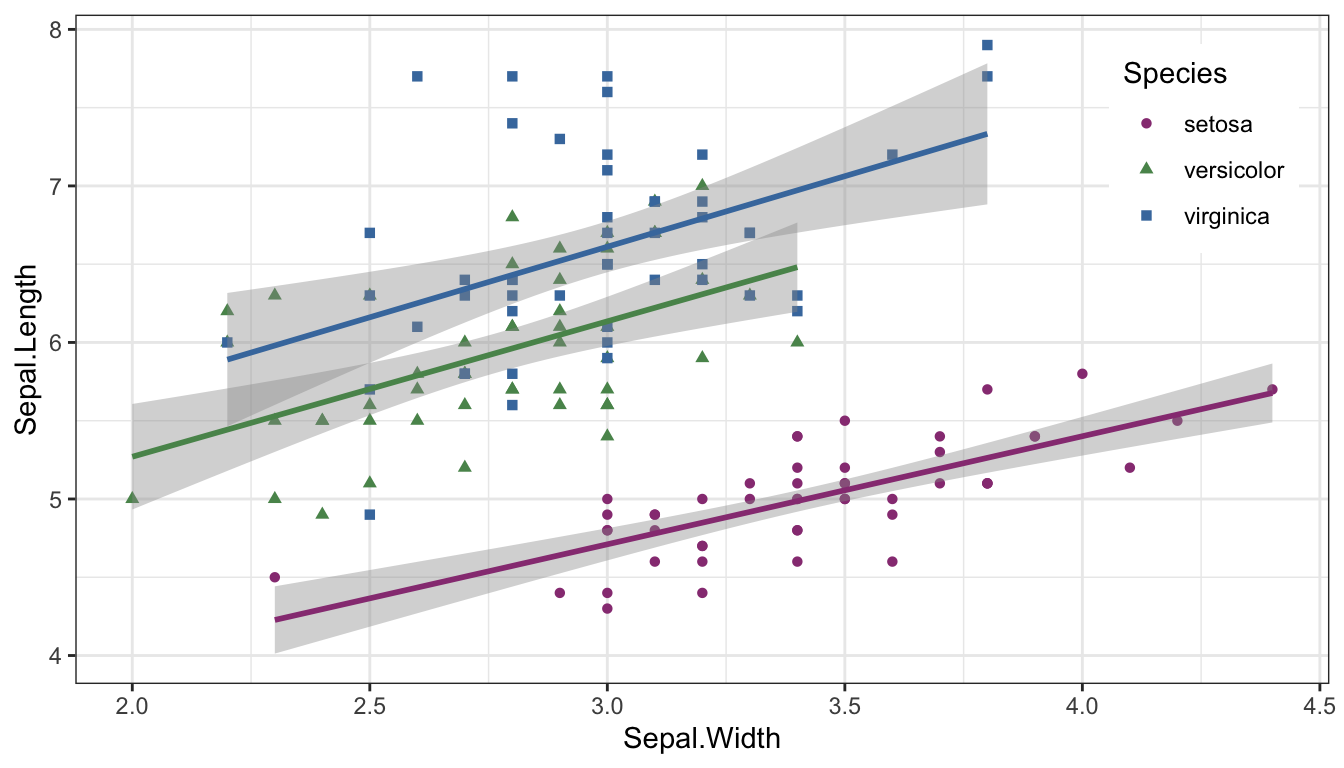
\includegraphics[width=1\linewidth]{01-intro_files/figure-latex/plot-shapes-1} 

}

\caption{Supplement point colours with shapes.}\label{fig:plot-shapes}
\end{figure}

\hypertarget{sex-gender-and-sexuality}{%
\section{Sex, gender and sexuality}\label{sex-gender-and-sexuality}}

When teaching about experimental design, sex always used to be my go-to example of a two-level between-subjects factor. But this can make some people feel like their very existence is being ignored. In your examples, avoid implicitly assuming heterosexuality or binary gender.

If you want to suggest an in-class exercise that uses data from the students, make sure to choose something that doesn't exclude anyone.

\begin{itemize}
\tightlist
\item
  Pet owners/non-pet owners
\item
  Normally does/doesn't wear glasses
\item
  Can/can't juggle
\item
  Native/non-native English speakers
\item
  Born in Scotland/elsewhere
\end{itemize}

\hypertarget{appendix-appendices}{%
\appendix}


\hypertarget{installing-r}{%
\chapter{\texorpdfstring{Installing \texttt{R}}{Installing R}}\label{installing-r}}

Installing R and RStudio is usually straightforward. The sections below explain how and \href{https://www.youtube.com/watch?v=lVKMsaWju8w}{there is a helpful YouTube video here}.

\hypertarget{installing-base-r}{%
\section{Installing Base R}\label{installing-base-r}}

\href{https://cran.rstudio.com/}{Install base R}. Choose the download link for your operating system (Linux, Mac OS X, or Windows).

If you have a Mac, install the latest release from the newest \texttt{R-x.x.x.pkg} link (or a legacy version if you have an older operating system). After you install R, you should also install \href{http://xquartz.macosforge.org/}{XQuartz} to be able to use some visualisation packages.

If you are installing the Windows version, choose the ``\href{https://cran.rstudio.com/bin/windows/base/}{base}'' subdirectory and click on the download link at the top of the page. After you install R, you should also install \href{https://cran.rstudio.com/bin/windows/Rtools/}{RTools}; use the ``recommended'' version highlighted near the top of the list.

If you are using Linux, choose your specific operating system and follow the installation instructions.

\hypertarget{installing-rstudio}{%
\section{Installing RStudio}\label{installing-rstudio}}

Go to \href{https://www.rstudio.com/products/rstudio/download/\#download}{rstudio.com} and download the RStudio Desktop (Open Source License) version for your operating system under the list titled \textbf{Installers for Supported Platforms}.

\hypertarget{rstudio-settings}{%
\section{RStudio Settings}\label{rstudio-settings}}

There are a few settings you should fix immediately after updating RStudio. Go to \textbf{\texttt{Global\ Options...}} under the \textbf{\texttt{Tools}} menu (⌘,), and in the General tab, uncheck the box that says \textbf{\texttt{Restore\ .RData\ into\ workspace\ at\ startup}}. If you keep things around in your workspace, things will get messy, and unexpected things will happen. You should always start with a clear workspace. This also means that you never want to save your workspace when you exit, so set this to \textbf{\texttt{Never}}. The only thing you want to save are your scripts.

You may also want to change the appearance of your code. Different fonts and themes can sometimes help with visual difficulties or \href{https://datacarpentry.org/blog/2017/09/coding-and-dyslexia}{dyslexia}.

\begin{figure}

{\centering 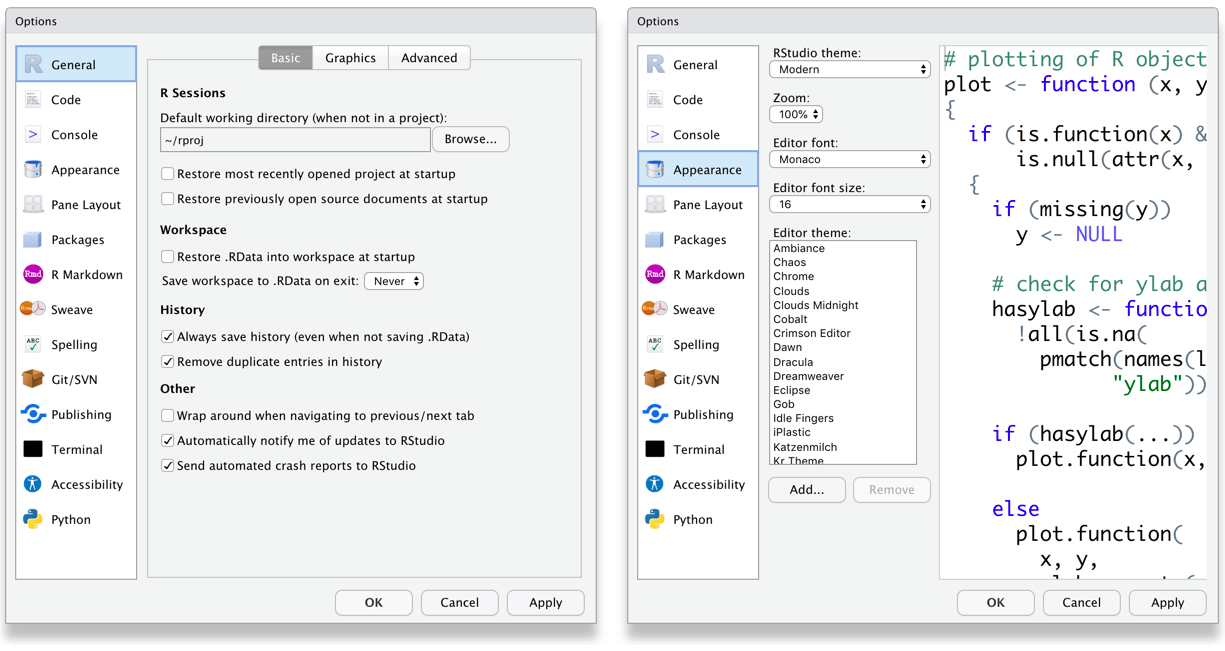
\includegraphics[width=1\linewidth]{images/rstudio_settings_general_appearance} 

}

\caption{RStudio General and Appearance settings}\label{fig:settings-general}
\end{figure}

You may also want to change the settings in the Code tab. Foe example, Lisa prefers two spaces instead of tabs for my code and likes to be able to see the whitespace characters. But these are all a matter of personal preference.

\begin{figure}

{\centering 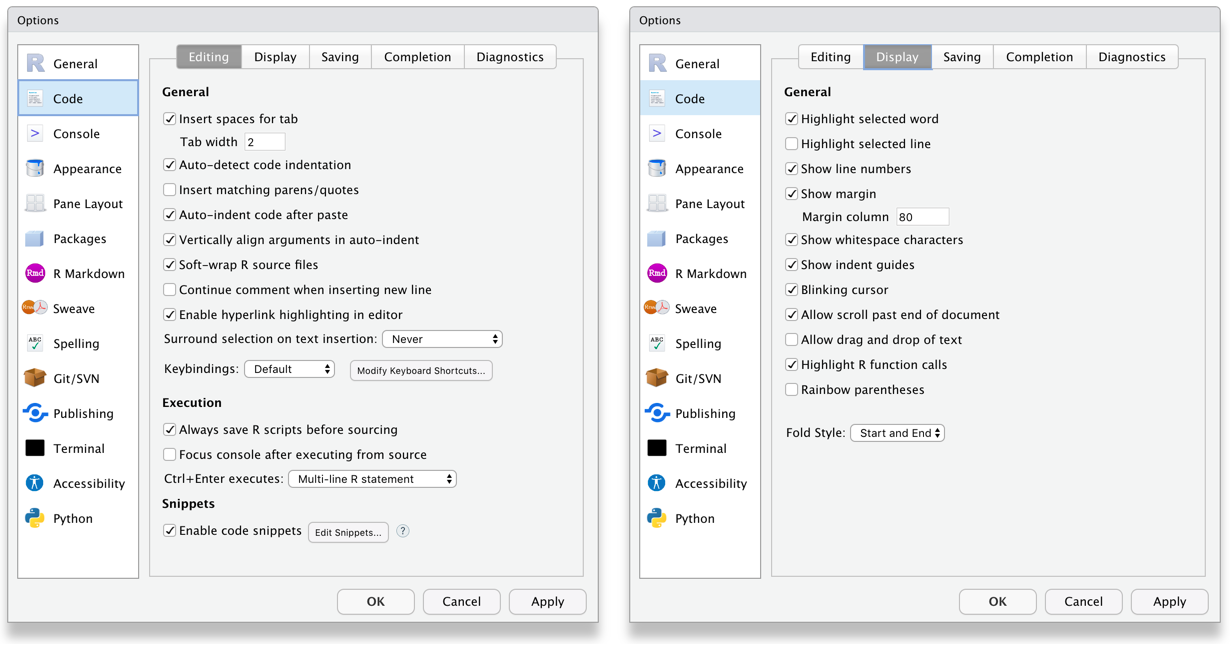
\includegraphics[width=1\linewidth]{images/rstudio_settings_code} 

}

\caption{RStudio Code settings}\label{fig:settings-code}
\end{figure}

\hypertarget{installing-latex}{%
\section{Installing LaTeX}\label{installing-latex}}

You can install the LaTeX typesetting system to produce PDF reports from RStudio. Without this additional installation, you will be able to produce reports in HTML but not PDF. This course will not require you to make PDFs. To generate PDF reports, you will additionally need to install tinytex \citep{R-tinytex} and run the following code:

\begin{Shaded}
\begin{Highlighting}[]
\NormalTok{tinytex}\SpecialCharTok{::}\FunctionTok{install\_tinytex}\NormalTok{()}
\end{Highlighting}
\end{Shaded}

\hypertarget{symbols}{%
\chapter{Symbols}\label{symbols}}

\begin{longtable}[]{@{}cll@{}}
\toprule
Symbol & psyTeachR Term & Also Known As \\
\midrule
\endhead
() & (round) brackets & parentheses \\
{[}{]} & square brackets & brackets \\
\{\} & curly brackets & squiggly brackets \\
\textless\textgreater{} & chevrons & angled brackets / guillemets \\
\textless{} & less than & \\
\textgreater{} & greater than & \\
\& & ampersand & ``and'' symbol \\
\# & hash & pound / octothorpe \\
/ & slash & forward slash \\
\textbackslash{} & backslash & \\
- & dash & hyphen / minus \\
\_ & underscore & \\
* & asterisk & star \\
\^{} & caret & power symbol \\
\textasciitilde{} & tilde & twiddle / squiggle \\
= & equal sign & \\
== & double equal sign & \\
. & full stop & period / point \\
! & exclamation mark & bang / not \\
? & question mark & \\
' & single quote & quote / apostrophe \\
" & double quote & quote \\
\%\textgreater\% & pipe & magrittr pipe \\
\textbar{} & vertical bar & pipe \\
, & comma & \\
; & semi-colon & \\
: & colon & \\
@ & ``at'' symbol & \href{https://www.theguardian.com/notesandqueries/query/0,5753,-1773,00.html}{various hilarious regional terms} \\
\ldots{} & \texttt{glossary("ellipsis")} & dots \\
\bottomrule
\end{longtable}

\begin{figure}

{\centering 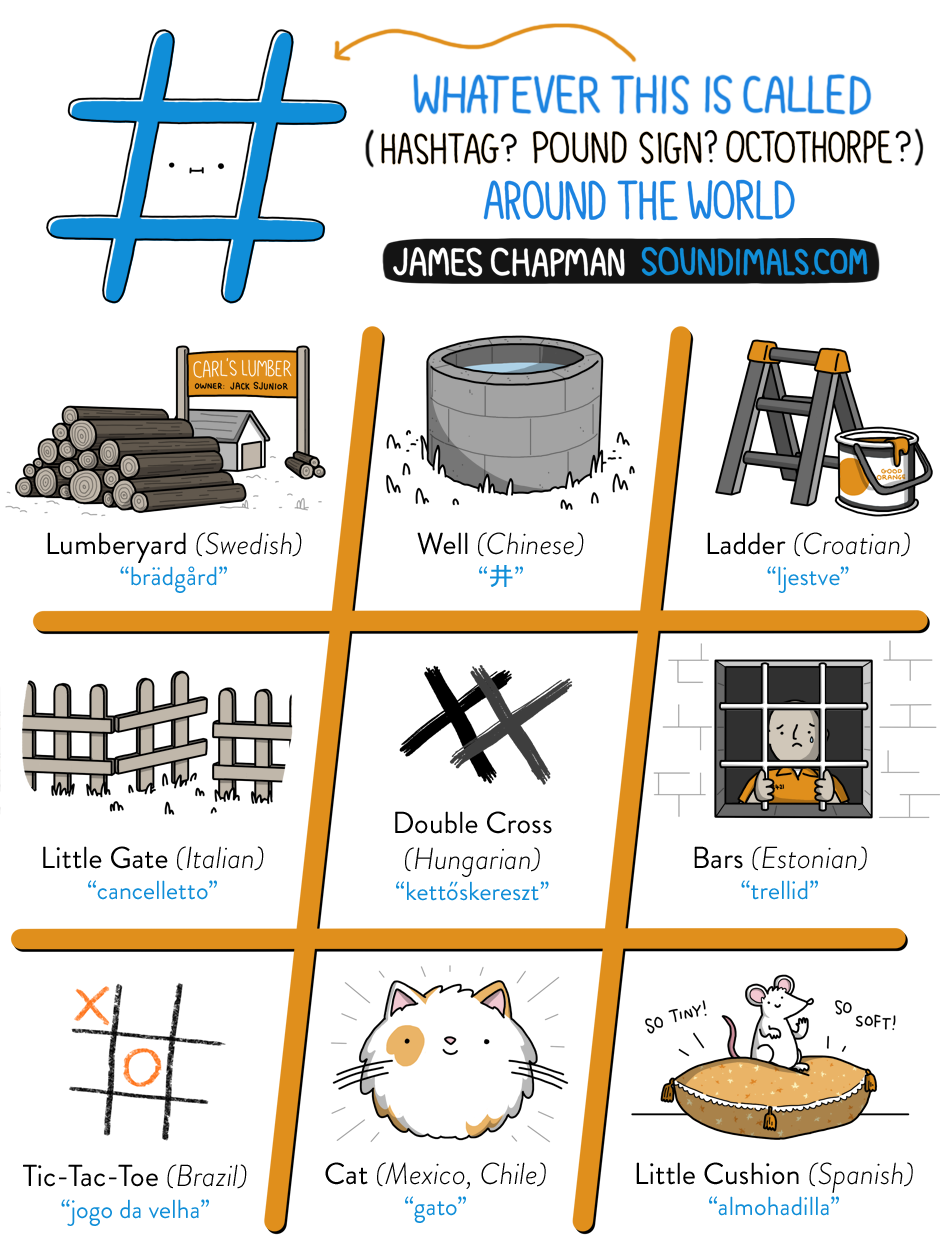
\includegraphics[width=1\linewidth]{images/soundimals_hash} 

}

\caption{[Image by James Chapman/Soundimals](https://soundimals.tumblr.com/post/167354564886/chapmangamo-the-symbol-has-too-many-names)}\label{fig:img-soundimals-hash}
\end{figure}

\hypertarget{conventions}{%
\chapter{Conventions}\label{conventions}}

This book will use the following conventions:

\begin{itemize}
\tightlist
\item
  Generic code: \texttt{list(number\ =\ 1,\ letter\ =\ "A")}
\item
  Highlighted code: {dplyr}{::}{slice\_max}{(}{)}
\item
  File paths: data/sales.csv
\item
  R Packages: tidyverse
\item
  Functions: {paste}{(}{)}
\item
  Strings: {``psyTeachR''}
\item
  Numbers: {100}, {3.14}
\item
  Logical values: {TRUE}, {FALSE}
\item
  Glossary items: ordinal
\item
  Citations: \citet{R-tidyverse}
\item
  Internal links: Chapter~\ref{inclusion}
\item
  External links: \href{https://r4ds.had.co.nz/}{R for Data Science}
\item
  Menu/interface options: \textbf{\texttt{New\ File...}}
\end{itemize}

\hypertarget{webexercises}{%
\section{Webexercises}\label{webexercises}}

See \href{https://psyteachr.github.io/webexercises/}{webexercises} for more details about how to use this in your materials.

\begin{itemize}
\tightlist
\item
  Type an integer:
\item
  I am going to learn a lot: TRUEFALSE
\item
  What is a p-value?

  \hypertarget{radio_LLQBBPYUJJ}{}
  {the probability that the null hypothesis is true} {the probability of the observed (or more extreme) data, under the assumption that the null-hypothesis is true} {the probability of making an error in your conclusion}
\end{itemize}

Hidden Text

You found some hidden text!

Hidden Code

\begin{Shaded}
\begin{Highlighting}[]
\FunctionTok{print}\NormalTok{(}\StringTok{"You found some hidden code!"}\NormalTok{)}
\end{Highlighting}
\end{Shaded}

\begin{verbatim}
## [1] "You found some hidden code!"
\end{verbatim}

\hypertarget{alert-boxes}{%
\section{Alert boxes}\label{alert-boxes}}

\begin{info}
Informational asides.

\end{info}

\begin{warning}
Notes to warn you about something.

\end{warning}

\begin{dangerous}
Notes about things that could cause serious errors.

\end{dangerous}

\begin{try}
Try it yourself.

\end{try}

\hypertarget{code-chunks}{%
\section{Code Chunks}\label{code-chunks}}

\begin{Shaded}
\begin{Highlighting}[]
\CommentTok{\# code chunks}
\FunctionTok{paste}\NormalTok{(}\StringTok{"Applied"}\NormalTok{, }\StringTok{"Data"}\NormalTok{, }\StringTok{"Skills"}\NormalTok{, }\DecValTok{1}\NormalTok{, }\AttributeTok{sep =} \StringTok{" "}\NormalTok{)}
\end{Highlighting}
\end{Shaded}

\begin{verbatim}
## [1] "Applied Data Skills 1"
\end{verbatim}

\begin{Shaded}
\begin{Highlighting}[]
\CommentTok{\# code chunks with visible r headers}
\FunctionTok{library}\NormalTok{(tidyverse)}
\end{Highlighting}
\end{Shaded}

\hypertarget{glossary}{%
\section{Glossary}\label{glossary}}

\begin{tabular}{l|l}
\hline
term & definition\\
\hline
ordinal & Discrete variables that have an inherent order, such as number of legs\\
\hline
\end{tabular}

\hypertarget{glossary-1}{%
\chapter{Glossary}\label{glossary-1}}

You can use the \texttt{glossary()} function to automatically link to a term in the \href{https://psyteachr.github.io/glossary/}{psyTeachR glossary} or make your own project-specific glossary.

This will create a link to the glossary and include a tooltip with a short definition when you hover over the term. Use the following syntax in inline r: \texttt{glossary("word")}. For example, common data types are integer, double, and character.

If you need to link to a definition, but are using a different form of the word, add the display version as the second argument (\texttt{display}). You can also override the automatic short definition by providing your own in the third argument (\texttt{def}). Add the argument \texttt{link\ =\ FALSE} if you just want the hover definition and not a link to the psyTeachR glossary.

\begin{Shaded}
\begin{Highlighting}[]
\FunctionTok{glossary}\NormalTok{(}\StringTok{"data type"}\NormalTok{, }
         \AttributeTok{display =} \StringTok{"Data Types"}\NormalTok{, }
         \AttributeTok{def =} \StringTok{"My custom definition of data types"}\NormalTok{, }
         \AttributeTok{link =} \ConstantTok{FALSE}\NormalTok{)}
\end{Highlighting}
\end{Shaded}

{[}1{]} ``Data Types''

You can add a glossary table to the end of a chapter with the following code. It creates a table of all terms used in that chapter previous to the \texttt{glossary\_table()} function. It uses \texttt{kableExtra()}, so if you use it in a code chunk, set \texttt{results=\textquotesingle{}asis\textquotesingle{}}.

\begin{Shaded}
\begin{Highlighting}[]
\FunctionTok{glossary\_table}\NormalTok{()}
\end{Highlighting}
\end{Shaded}

\begin{tabular}{l|l}
\hline
term & definition\\
\hline
character & A data type representing strings of text.\\
\hline
data-type & My custom definition of data types\\
\hline
double & A data type representing a real decimal number\\
\hline
integer & A data type representing whole numbers.\\
\hline
\end{tabular}

If you want to contribute to the glossary, fork the \href{https://github.com/PsyTeachR/glossary}{github project}, add your terms and submit a pull request, or suggest a new term at the \href{https://github.com/PsyTeachR/glossary/issues}{issues page}.

\hypertarget{license}{%
\chapter*{License}\label{license}}
\addcontentsline{toc}{chapter}{License}

This book is licensed under Creative Commons Attribution-ShareAlike 4.0 International License \href{https://creativecommons.org/licenses/by-sa/4.0/}{(CC-BY-SA 4.0)}. You are free to share and adapt this book. You must give appropriate credit \citep{psyteachr-template}, provide a link to the license, and indicate if changes were made. If you adapt the material, you must distribute your contributions under the same license as the original.

  \bibliography{book.bib,packages.bib}

\end{document}
